% !TEX root =  ../FinalReport.tex

\chapter{Implementation}
\label{sec:Implementation} 

\section{Library Selection}
\label{sec:LibrarySelection}
\begin{figure}[ht]
    \centering
    \begin{tabular}{r|c c}
        & OpenGL & Vulkan \\
        \hline
        OpenCL & Y & N \\ 
        CUDA & Y & Y \\ 
        OpenGL & Y & N \\ 
        Vulkan & N & Y \\ 
    \end{tabular}
    \caption{Graphics and Compute Backend Interoperability Matrix}
    \label{fig:LibraryChoices}
\end{figure}
CUDA and Vulkan had already been highlighted in the Specification as likely choices of backends, but to be complete other backends were also considered.
As the simulation would have to run on DCS systems (\cref{reqN:DCSCompile}), and thus run on Linux, the only possible GPU rendering backends were OpenGL and Vulkan.
However there were still multiple choices of compute backend:
\begin{itemize}
    \item OpenCL\cite{tool:OpenCL1.0PressRelease} is an ``Open Standard for Parallel Programming of Heterogeneous Systems''\cite{TheKhronosGroupOpenCLInc}.
    \item CUDA\cite{tool:CUDA} is a closed-source library for running parallel code on NVIDIA GPUs.
    \item OpenGL has Compute Shaders\cite{tool:OpenGLComputeShaderExt} which can execute computations outside of the graphics pipeline.
    \item Vulkan also has Compute capability\cite{KhronosVulkanGuide}, similar in function to OpenGL.
\end{itemize}
To decide on the compute backend to use, an interoperability matrix was drawn (\cref{fig:LibraryChoices}) to show which libraries could share data without copying it between buffers.
As the researcher was already experienced with Vulkan, and the more granular control it provides would be beneficial to performance, Vulkan was selected as the rendering backend.
This prevented OpenCL and OpenGL from being used as compute backends, as they are not compatible with Vulkan.
CUDA and Vulkan have comparable ability, but CUDA was chosen as the compute backend.
The Vulkan compute shaders are still a very graphics-oriented view of computation, and CUDA would give the researcher experience with other kinds of libraries.
A Vulkan compute backend may still be used for the visualization portion of the code.

% Not for now, but note that the C++ vulkan bindings are nice. They do end up wrapped in other classes, but they remove the need to remember boilerplate as much.

In other cases there were clear choices: the SDL2\cite{SimpleHomepage} window and input library and the Dear ImGUI\cite{CornutDearImGui} UI library were chosen due to personal experience.
The \texttt{stb\_image.h} header was found to be a simple method of importing image color data as byte arrays, used for the input generator (\cref{req:GenerateState}).

There are a great many options for Command-Line parsing libraries, even more so because C++ is used instead of C.
A recent survey of the possibilities\cite{attractivechaos2018AC/C++} was whittled down to five options.

\texttt{getopt}\cite{FreeSoftwareFoundationGetopt3:Page}, \texttt{argp}\cite{GNUProjectArgpLibrary}, and \texttt{gopt}\cite{VajzovicGoptLibrary} are C libraries that use arrays of structures to define the required arguments.
Of them, only \texttt{argp} can automatically generate a \texttt{--help} argument, which is a very valuable feature.

\texttt{cxxopts}\cite{jarro2783Cxxopts:Parser} was considered as a C++ alternative, but used very odd syntax for defining arguments.
Ultimately CLI11\cite{CLIUtilsCLI11} was chosen as a modern C++11 library that had native support for subcommands, which were used heavily for separating program components (see \cref{sec:DesignSubcommands}).

\section{Build System}
The build system is implemented in CMake\cite{tool:Cmake} as specified in \cref{sec:ProjManagementTools}.
This section highlights a few changes that were made to an otherwise standard setup to accommodate the project.

\subsection{CUDA-less Binaries}
The project can be built to produce both CUDA and CUDA-less binaries, in case it needs to be run on CUDA-less computers.
The list of regular C++ source files and CUDA source files are maintained separately. A CUDA-less binary (\texttt{sim\_nocuda}) will only build the C++ files while a CUDA binary (\texttt{sim\_cuda}) will build both.
When building the \texttt{sim\_cuda} target the preprocessor macro \texttt{CUDA\_ENABLED} is defined throughout all source files, including the C++ files.
This allows support for CUDA backends in C++ code (i.e. as selectable options on the command-line) to be conditionally enabled without maintaining two copies of the relevant source files.
In \cref{fig:ConditionalCUDA} (which has been amended for brevity), the switch statement only contains a case for CUDA if the directive is set, triggering a fatal error otherwise.
\begin{figure}[ht]
    \centering
\begin{cppcode}
switch(backendType) {
    case Null:
        return SimFixedTimeRunner<NullSimulation, Host2DAllocator>();
    case CpuSimple:
        return SimFixedTimeRunner<CpuSimpleSimBackend, Host2DAllocator>();
    case CpuOptimized:
        return SimFixedTimeRunner<CpuOptimizedSimBackend, Host2DAllocator>();
    case CpuAdapted:
        return SimFixedTimeRunner<CpuOptimizedAdaptedSimBackend, Host2DAllocator>();
#if CUDA_ENABLED
    case CUDA:
        return SimFixedTimeRunner<CudaBackendV1<true>, CudaUnified2DAllocator>();
#endif
    default:
        FATAL_ERROR("Enum val %d doesn't have an ISimFixedTimeRunner!\n", backendType);
}\end{cppcode}
\caption{Conditionally supporting CUDA based on a preprocessor directive}
    \label{fig:ConditionalCUDA}
\end{figure}


\subsection{Shader Build Infrastructure} % Fits in with the build system vibe
The shaders used for visualization are written in GLSL, with appropriate extensions to be compatible with Vulkan.
They are separated by file type, with Vertex shaders in \texttt{.vert} files and Fragment shaders in \texttt{.frag} files.
As Vulkan does not natively support GLSL, they must be compiled to SPIR-V before they can be used.
CMake does not support GLSL as a first-class language, so a custom build command was used to compile them with \texttt{glslc}\cite{GoogleLLCShaderc} when they change.
This allows them to be treated just like any other source file from the programmer's perspective.
The SPIR-V files are placed in a \texttt{shaders} directory next to the binaries, where they can be easily accessed and passed to Vulkan.

\section{Memory Usage}
The CUDA simulation backend makes use of CUDA Unified Memory\cite{Harris2017UnifiedBlog} whenever possible.
This allows the memory to be accessed from the CPU and the GPU without having to manually map it, and instead pages the memory between devices on request.
Once the pages are on the GPU, it can be accessed with the same speed as manually allocated GPU memory.
The main benefit of this is that any functionality that has not yet been implemented on the GPU, or that may be faulty, can be easily replaced with pre-existing CPU code to verify the simulation correctness.
Moving memory between the CPU \& GPU does decrease performance, as any memory movement would, but as it is only intended for development this is OK.

% TODO - text wrapping for external memory
Memory that needs to be shared between CUDA and Vulkan is allocated through Vulkan and then mapped to a CUDA pointer via the \texttt{VK\_KHR\_external\_memory\_fd} Vulkan extension\cite{tool:VulkanKHRExternalMemoryFD} and the CUDA External Memory API\cite{NVIDIAExternalInteroperability}.
It is possible for memory to be imported from CUDA into Vulkan, but allocating through Vulkan gives more control over where memory is allocated.
Because of the limited flexibility of Vulkan-controlled memory compared to Unified Memory, this is used sparingly and only for data that absolutely must be shared between the APIs.

Vulkan memory is only used when Vulkan is present i.e. during the real-time visualization.
In the headless mode, all of the memory is CUDA Unified Memory.
This could lead to problems if the simulation assumes memory is Unified and CPU-accessible when it would be Vulkan memory during the visualization.
In this case the code would break only during the real-time visualization when the pointer is accessed, and not during the headless simulation.
To avoid this, a templated smart-pointer class \texttt{CUDAUnified2DArray<class T, bool IsUnified>} is used for each pointer to CUDA-usable memory.
This automatically frees the memory when possible, and provides \texttt{as_gpu()} and \texttt{as_cpu()} functions which the programmer uses to access the data.
C++ \texttt{static_assert} and \texttt{if constexpr} logic is used to create a compilation error when non-Unified memory is accessed through \texttt{as_cpu()}, preventing the issue from ever occurring.

\begin{figure}[ht]
    \centering
    \lstset{language=c++,
    morekeywords={constexpr},
    keywordstyle=[2]\color{blue},
    keywords=[2]{OriginalOptimized,CudaUnified2DArray}
    % literate=
    %         *{\{}{{\textcolor{myblue}{\{}}}{1}
}%[language=c++]
    \begin{lstlisting}
if constexpr (UnifiedMemoryForExport) {
    // The buffer is Unified Memory, so use it directly
    OriginalOptimized::splitToRedBlack(p.joined.as_cpu(),
                                       p_buffered.red.as_cpu(),
                                       p_buffered.black.as_cpu(),
                                       imax, jmax);
} else {
    // The buffer is not unified memory, 
    // so create a new Unified memory buffer and copy the data in,
    // then use that instead.
    CudaUnified2DArray<float, true> p_unified(unifiedAlloc.get(), matrix_size);
    p_unified.memcpy_in(p.joined);
    OriginalOptimized::splitToRedBlack(p_unified.as_cpu(),
                                       p_buffered.red.as_cpu(),
                                       p_buffered.black.as_cpu(),
                                       imax, jmax);
}\end{lstlisting}
    \caption{An example of conditionally changing code based on memory type.}
    \label{fig:TemplatedMemoryUsage}
\end{figure}
The CUDA backend itself is also templated on whether it is being run with Vulkan-exported memory.
This allows simulation code to detect whether the memory would be CPU-accessible or not, and take action accordingly.
In \cref{fig:TemplatedMemoryUsage}, this is used to conditionally copy data into a Unified Memory buffer so that it can be used with a part of the algorithm that has not yet been implemented on the GPU.
If the memory is already Unified, the copy is skipped, but if the memory is Vulkan-based the copy is performed to prevent a SEGFAULT.
This logic uses \texttt{if constexpr}, so all branches are eliminated at compile-time adding a very slight performance boost.

\section{Current Status}
\label{sec:ImplementationCurrentStatus}
The \texttt{makeinput}, \texttt{compare}, and \texttt{renderppm} subcommands are all functional.
More functionality may be added if necessary for efficient development, and potential changes have been outlined in the previous sections.

The \texttt{fixedtime} headless simulation is functional, with each backend performing as intended. More optimization is intended (\cref{sec:Research:Optimization}), but the current program is fast enough to simulate the original ACA input at 120 ticks per second\footnote{On the researcher's GTX 1080. The program hasn't been tested on other systems.} which is a good baseline.

\begin{figure}[ht]
    \centering
    \centerline{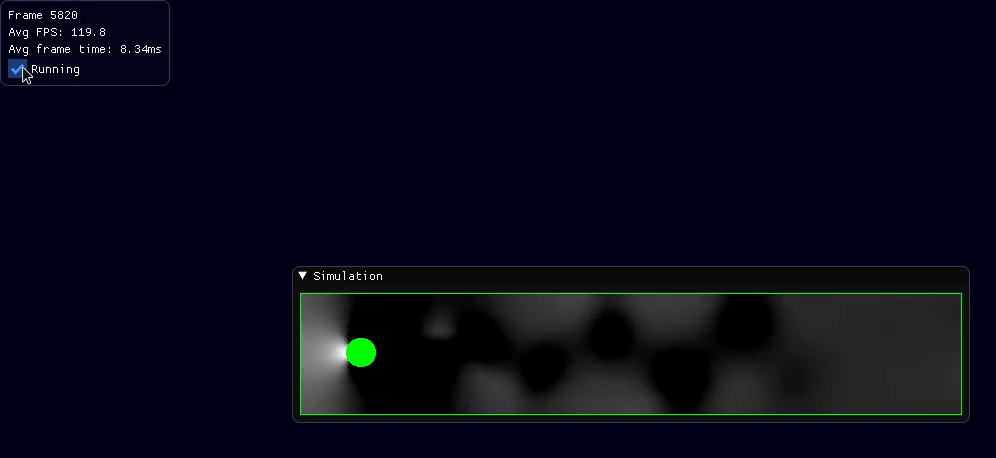
\includegraphics[width=1.25\linewidth]{Ch48Implementation/figures/example_running.png}}
    \caption{An example of the real-time visualization running on the ACA input}
    \label{fig:ExampleRunning}
\end{figure}
The visualized simulation creates a 1280x720 window and displays the simulation in a subwindow, which the user can move around.
The visualization is a simple display of the current pressure values, which is subpar (see \cref{sec:VizPressureCritique}), but this is planned to change.
A second window displays statistics about the last frame, and shows a checkbox which controls if the simulation is running as per \cref{req:VizPauseResume}.
As seen in this window, the simulation is running at 120 frames per second.
Each simulation tick is 1/60th of a second of simulation time, so the simulation is running at 2x real time.
This will be changed to account for \cref{req:VizSomeSpeed}.

